\documentclass{article}
\usepackage[utf8]{inputenc}
\usepackage[T1]{fontenc}
\usepackage[spanish]{babel}
\usepackage{setspace}
\usepackage{geometry}
\geometry{margin=2.5cm}
\setstretch{1.2}
\usepackage{graphicx}
\usepackage[utf8]{inputenc}
\usepackage[spanish]{babel}
\usepackage{amsmath}
\usepackage{float}
\usepackage[utf8]{inputenc}
\usepackage[spanish,mexico]{babel}
\usepackage[margin=2.5cm]{geometry}
\usepackage{graphicx}
\usepackage[export]{adjustbox}
\usepackage{caption}
\usepackage{subcaption}
\usepackage{fancyhdr}
\usepackage{enumitem}
\usepackage{amsmath}
\usepackage{amssymb}
\usepackage{amsfonts}
%\usepackage{hyperref}
\usepackage[colorlinks=true, allcolors=blue]{hyperref}
\pagestyle{fancy}
\fancyhf{}

\usepackage[T1]{fontenc}   
    \usepackage{array}
    \newcommand{\tarjeta}[3]{%
      \begin{center}
      \begin{tabular}{|>{\raggedright\arraybackslash}p{7.8cm}|>{\raggedright\arraybackslash}p{4.2cm}|}
        \hline
        \multicolumn{2}{|c|}{#1} \\ \hline
        #2 & #3 \\ \hline
      \end{tabular}
      \end{center}
    }
\title{Template Facultad de Ciencias, UNAM}
\author{Yoltic Giovanni Santillan Ruiz}


\begin{document}

\thispagestyle{empty}
	
	\begin{figure}[ht]
	   \minipage{0.76\textwidth}
			
\includegraphics[width=4cm]{Logo_UNAM.png}
			\label{EscudoUNAM}
	   \endminipage
	   \minipage{0.32\textwidth}
			
\includegraphics[height=4.3cm ,width=4.3cm]{Logo_FC.png}
			\label{EscudoFC}
		\endminipage
	\end{figure}
	
	\begin{center}
	\vspace{0.8cm}
	\LARGE
	UNIVERSIDAD NACIONAL AUTÓNOMA DE MÉXICO 
	
	\vspace{0.8cm}
	\LARGE
	FACULTAD DE CIENCIAS
	
	\vspace{1.7cm}	
	\Large
	\textbf{Proyecto 2 Rocola}

	\vspace{1.3cm}
	\normalsize	
	PRESENTA \\
	\vspace{.3cm}
	\large
	\textbf{Yoltic Giovanni Santillan Ruiz \\ 323124539}
	
	\end{center}
	
	\newpage



\section{Resumen}
\label{sec:resumen}

Este proyecto es una aplicacion para el manejo de archivos mp3 con etiqueta id3v2.4, donde puedes editar el titulo, album, artista, etc, ademas de poder reproducir la musica, todo esto con una base de datos. Utilice C\#\ como lenguaje de programacion, Avalonia UI \cite{avalonia} (patrón MVVM \cite{mvvm}), SQLite \cite{sqlite} (base de datos), LibVLCSharp \cite{libvlcsharp} (reproducción de audio) y TagLibSharp \cite{taglibsharp} (lectura de etiquetas).

El proyecto se compone de 3 partes principalmente, la interfaz grafica (Con lo que el usuario interactua), el minero (Obtiene la informacion de la base de datos), la base de datos (Donde se guarda la informacion de los mp3) 
\section{Introducción}
\label{sec:introduccion}

\subsection{Problema a resolver}
A toda persona en este mundo le gusta la musica, pero a nadie le gusta navegar entre tus archivos para poder reproducirla, asi que esta aplicacion te ayuda a organizar y usar de manera mas amigable, en el mercado hay algunas aplicaciones, pero son de paga o tienen anuncios o necesitas internet, esta es una aplicacion lligera, que no necesita internet y de codigo abierto

\subsection{Alcance}
Si el usuario tiene su musica descargada la experiensia es buena, ya  al no necesitar conexion puedes usarla en cualquier lado

\subsection{Limitaciones y posibles problemas}
La principal limitacion es qeu el usuario debe tener su musica con etiquetas id3v2.4 descargada y esto puede ser poco dificil pues actualmente ya no se acostumbra a tener esto pues todo se hace por internet, pero si el usuario se da a la tarea de hacerlo la experiencia es buena

\subsection{Mejoras}

Hay varias cosas por mejorar, como una barra para poder regresar adelantar y regresar a una cancion, que la aplicacion muestre las portadas de las canciones y de los albums, tambien mejorar la busqueda, la que el programa tiene cumple, sin embargo podria llegar a ser mejor
\section{Análisis y diseño}
\label{sec:analisis-y-diseno}

 Aunque ya habia trabajado con C\#\ al inciar el proyecto no tenia nada de experiencia con base de datos ni con las etiquetas id3v2.4, asi que el diseño fue construido un poco a ciegas, pero se dividio en los siguientes subproblemas
 
\subsection{Minero}

\subsubsection{Division en subproblemas}

\begin{itemize}
    \item \textbf{¿Cómo buscar los archivos mp3?}

    \item \textbf{¿Cómo leer las etiquetas id3v2.4?}

    \item \textbf{¿Donde guardar la informacion de los mp3?}

    \item \textbf{¿Como crear la base de datos?}

    \item \textbf{¿Cómo meter la informacion a la base de datos?}

\end{itemize}

\subsubsection{Respuestas a los subproblemas}

\begin{itemize}
    \item Usando la libreria System.IO podemos buscar en un directorio archivos con una terminacion especifica

    \item Con la libreria ya que filtramos los archivos con terminacion mp3 abrimos la etiqueta con la libreria TagLibSharp \cite{taglibsharp} para ver si es id3v2.4 y obtener los datos
    
    \item Lo mejor era crear un objeto Ficha por cada mp3 leido con todas las propiedades que obteniamos de la etiqueta y meterlos en una lista de Ficha, para tener todos los datods en un mismo lugar
    
    \item El sistema utiliza una base de datos con SQLite \cite{sqlite}. El método conectar() verifica la existencia del archivo musica.db; si no existe, lee y ejecuta un script SQL (rolas.sql que es el que mando Canek en el correo) que contiene la definición de las tablas.
    
    \item Iteramos la lista de Fichas y con ayuda de la libreria Microsoft.Data.Sqlite \cite{microsoftsqlite} vamos insertando en la base, pero verificamos por cada cancion que su artista o el album existen, para no repetir datos, ademas verficamos por la ruta de cada archivo para no repetir canciones

\end{itemize}


La Figura~\ref{fig:flujoMinero} muestra el flujo del minado el proceso inicia recibiendo la carpeta a minar y verificando que exista. Se crea una lista de Fichas que se llena leyendo la etiqueta exactamente id3v2.4 de cada archivo MP3 encontrado. Una vez terminada la lectura, se verifica si el archivo de la base de datos existe; si no, se crea. Finalmente, por cada canción, se comprueba en la base de datos si el artista y el álbum ya existen (para evitar duplicados) y, de ser necesario, se insertan antes de agregar la canción a la tabla principal.


\begin{figure}[H]
    \centering
    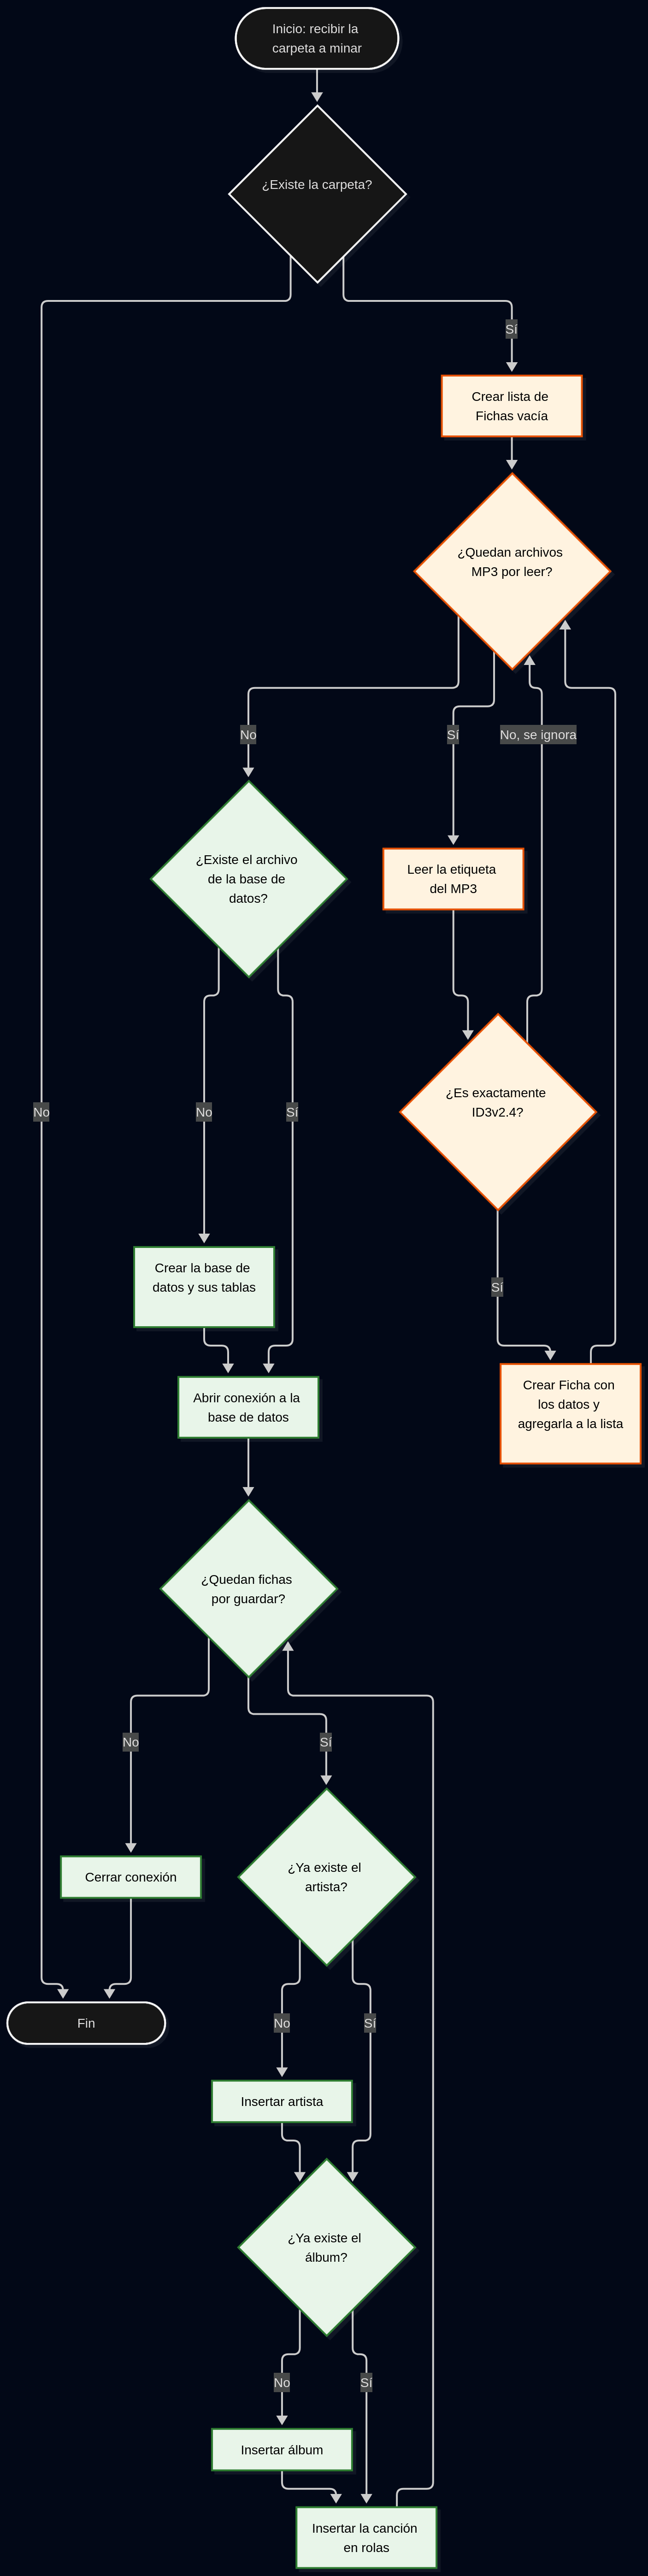
\includegraphics[height=0.9\textheight, keepaspectratio]{flujoMinero.png}
    \caption{Diagrama de secuencia del flujo MINAR.}
    \label{fig:flujoMinero}
\end{figure}

\subsubsection{Cronología}

  Lo primero que hice fue ejecutar dotnet para crear un nuevo proyecto; desde un inicio lo separé siguiendo el patrón MVC. Revise cómo buscar archivos MP3 en un directorio, y de ahí ver cómo leer las etiquetas con TagLib. Al inicio traté de leer los bits a mano, pero era muy complicado y tardado, así que mejor busqué una librería, ya que Canek mencionó que hacerlo a mano era muy tonto, pues nos iba a llevar mucho tiempo. Después creé el objeto Ficha para guardar la información obtenida de las etiquetas, y posteriormente investigué cómo funcionaba Microsoft.Data.Sqlite para meter la información a la base de datos.
  
\subsubsection{Notas}

\begin{itemize}
    \item En un inicio habia hecho el minero como un ejecutable independiente, sin embargo al darme cuenta de que la interfaz tambien iba a hacer uso del minero lo pase a una libreria, afortunadamente como desde un incio habia seguido el patron MVC, esto no fue complicado, solo tuve que mover el modelo a la libreria, y asi el controlador y la vista se quedaron en el ejecutable del minero.
\end{itemize}


\subsubsection{Tarjetas CRC del Minero}

\tarjeta{Mina}
{Obtiene el directorio mediante los argumentos del main\newline
 Verifica que el directorio existe\newline
 Crea un nuevo Minero y manda a llamar minar() metodo de la biblioteca para empezar todo\newline
 Le avisa a la vista si todo sale bien o si hay algun error}
{Minero\newline
Vista}

\tarjeta{Vista}
{Imprime en pantalla lo que el controlador (Mina) le envie}
{Mina}

\subsubsection{Tarjetas CRC de la libreria del minero}
\tarjeta{Minero}
{Crear la lista de Ficha\newline
 Llamar al metodo procesar de MetaDatos pasandole el directorio recibido por el controlador y la lista recien creada\newline
 Hacer conexion a la base de datos con el metodo conectar() de BaseDeDatos\newline
 Agregar las canciones a la base de datos con el metodo agregar() de BaseDeDatos pasandole la lista de Fichas ya llena y la conexion}
{BaseDeDatos\newline MetaDatos\newline Ficha}

\tarjeta{Ficha}
{Objeto con propiedades obtenidas de las etiquetas:\newline
 titulo, genero, performer, album, track, year, apath, rpath}
{Minero}

\tarjeta{MetaDatos}
{Consigue todos los mp3 de el directorio\newline
 Crea las fichas con los datos de la etiqueta siempre y cuando sea id3v2.4\newline
 Regresa la lista con todas las Fichas}
{Minero}

\tarjeta{BaseDeDatos}
{Crear conexion con la base de datos o crearla sino existe\newline
 Agregar las canciones a la base de datos\newline
 Verfica si el artista y album ya existen para no repetir}
{Minero}

\subsection{Interfaz}

\subsubsection{Subproblemas}

\begin{itemize}
    \item \textbf{¿Como crear una interfaz?}

    \item \textbf{¿Como mostrar las canciones de la base de datos?}
    
    \item \textbf{¿Cómo crear los botones para que el usuario decida que hacer?}
    
    \item \textbf{¿Cómo obtener la informacion que el usuario escriba para modificar o agregar?}
    
    \item \textbf{¿Cómo actualizar las cosas en la base de datos?}
    
    \item \textbf{¿Cómo hacer la busqueda?}

    \item \textbf{¿Cómo recibir la ruta para la carpeta de musica?}
\end{itemize}

\subsubsection{Respuestas a los subproblemas}

\begin{itemize}
    \item Este fue el primer problema al que me enfrente pues la mayoria de interfaces en C\#\ son para  windows, asi que busque para Linux, asi que llegue a Avalonia ~\cite{avalonia}, creando mi interfaz con dotnet new avalonia.mvvn \cite{mvvm}, la cual sigue el patron modelo, vista, vista modelo que es como el controlador en MVC, usando AXAML para el diseño visual.
    
    \item Se necesita usar el patron Observer con la clase ObservableCollection<T> de .NET, la cual le avisa a la interfaz si algo cambia dentro de ella, pero primero consultamos la base de datos para crear los objetos CancionFila (con las propiedades titulo, genero, performer, album, id, id\_\ performer, id\_\ album, path) agregandolos en una lista, para despues pasarlos a la ObservableCollection, asi en el AXAML la enlazamos con el DataGrid para que muestre la informacion
    
    \item Aqui ocupe <Button> de Avalonia para crear un boton en la interfaz y para ver que hacia cada boton, ocupe 2 cosas distintas:
    
    -Command; para la logica pesada, como la busqueda avanzada, reproducir la musica, el boton se enlaza con el ViewModel con RelayCommand 

    -Click; para principalmente cosas visuales como abrir una nueva ventana o cerrar, cosas especificamente de la Vista, esto funciona agregando el metodo que se va a ejecutar cuando presionemos el boton.
    
    \item Para guardar la información que el usuario ingresa, ya sea para modificar o para agregar, le pasamos un objeto con las propiedades necesarias mediante el DataContext a la ventana. Gracias a que utilizamos Mode=TwoWay en las cajas de texto donde el usuario escribe, estas se enlazan automáticamente al objeto. Así, cuando el usuario presiona el botón de guardar, haciendo uso de Close(objeto) obtenemos el objeto con las propiedades ya cambiadas para enviarlo a la base de datos
    
    \item Una vez que tenemos el objeto con las propiedades modificadas, utilizamos la librería Microsoft.Data.Sqlite para actualizar o agregar los datos en la base de datos, aqui tomamos en cuenta que considerar para que dos registros sean iguales y asi no tener repeticion, se explica mejor en la nota
    
        
    \item Para la busqueda, puse un panel desplegable en la interfaz controlado por un booleano (MostrarPanelBusqueda), asi el usuario puede filtrar por título, artista, álbum y género. La captura de los criterios se realiza de la misma forma que en toda la interfaz con un objeto y enlaces Mode=TwoWay
    
    En la capa de datos, se implementó una consulta SQL dinámica. Se parte de una base con la cláusula WHERE 1=1 para facilitar la concatenación condicional. Por cada campo de texto que contenga información, se añade un AND columna LIKE @parametro, utilizando el comodín \%\ para permitir búsquedas parciales. Si una caja de texto está vacía, el filtro se ignora, lo que permite hacer búsquedas tan específicas o generales como el usuario desee.
    
    Finalmente, el ViewModel recibe los resultados, limpia la ObservableCollection y la llena con las coincidencias, haciendo que el DataGrid se actualice. Además, se incluyó un botón de 'Limpiar' que reinicia los filtros y recarga la biblioteca completa desde SQLite.

    \item Para recibir la ruta del minado, creé una nueva ventana que se abre cuando el usuario presiona el botón de minar. En esta ventana se muestra una caja de texto para que el usuario escriba la ruta. Así, haciendo uso de Close(texto), obtenemos el string de vuelta y lo enviamos a la librería para realizar el minado.
    
    \end{itemize}

\subsubsection{Cronología}
Primero entendí cómo funcionaba la interfaz y cómo se mostraban las cosas. Empecé con la ventana principal, viendo cómo mostrar las canciones y cómo hacer la barra de la canción actual. Después fui haciendo los botones y, conforme hacía cada uno, escribía el código y la lógica para que funcionaran. Lo último fue hacer la búsqueda y poder reproducir la música.

\subsubsection*{Nota sobre la validación de duplicados en Artistas y Álbumes}

Para evitar registros duplicados en la base de datos cuando el usuario edita un nombre, se establecieron criterios específicos para determinar cuándo dos entidades se consideran ``iguales'':

\begin{itemize}
    \item \textbf{Artistas (Performers):} A nivel general, se considera que un artista es el mismo si coincide su \textbf{nombre artístico} (\texttt{name}). Sin embargo, para ser más estrictos en las tablas específicas, se aplicaron las siguientes reglas:
    \begin{itemize}
        \item \textbf{Personas:} Se consideran iguales si coinciden tanto el \textbf{nombre artístico} (\texttt{stage\_name}) como el \textbf{nombre real} (\texttt{real\_name}).
        \item \textbf{Bandas:} Se consideran iguales si coinciden el \textbf{nombre de la banda} (\texttt{name}) y su \textbf{fecha de creación} (\texttt{start\_date}).
    \end{itemize}
    \item \textbf{Álbumes:} Se consideran iguales si coinciden únicamente por su \textbf{nombre}.
\end{itemize}

Si al momento de guardar los cambios el sistema detecta que el nuevo nombre ya existe bajo estos criterios, se activa la lógica de fusión (Merge): las canciones se reasignan al registro original y el registro duplicado se elimina.

\subsubsection{Tarjetas CRC de la Interfaz}

    \tarjeta{MainWindow (Vista Principal)}
    {Contiene el diseño visual y los eventos de la ventana principal.\newline
    AXAML: Define el \texttt{DataGrid} de canciones, la barra de reproducción (con botones de play/pausa y metadatos), el panel de búsqueda y la barra de botones superior.\newline
    C\#: Captura los clics de los botones. Evalúa el tipo de artista para abrir la ventana correspondiente (Persona, Banda o Desconocido). Utiliza \texttt{ShowDialog} para esperar asíncronamente los datos modificados de las ventanas secundarias y los envía al ViewModel para su actualización.}
    {MainWindowViewModel (Lógica de negocio)\newline
    Ventanas secundarias: MinarWindow, TituloWindow, PersonaWindow, BandaWindow, DesconocidoWindow, AlbumWindow, RegistrarArtistaWindow, AgregarPersonaWindow.\newline
    Modelos: Artista, Album, Titulo, CancionFila.}
    
    \tarjeta{RegistrarArtistaWindow (Ventana Secundaria)}
    {Actúa como un menú intermedio para cambiar el tipo de un artista.\newline
    AXAML: Muestra el nombre y tipo actual del artista (\texttt{TipoTexto}). Contiene botones para convertirlo en Persona, Banda o Desconocido.\newline
    C\#: Al hacer clic en una opción, abre la ventana de edición correspondiente (\texttt{RegistrarPersonaWindow}, \texttt{RegistrarBandaWindow} o \texttt{RegistrarDesconocidoWindow}) pasándole el objeto \texttt{Artista}.}
    {Modelo Artista\newline
    RegistrarPersonaWindow\newline
    RegistrarBandaWindow\newline
    RegistrarDesconocidoWindow\newline
    MainWindow (Ventana que la invoca)}
        

\tarjeta{MinarWindow (Ventana de Diálogo)}
{Ventana modal que solicita al usuario la ruta de una carpeta.\newline
AXAML: Proporciona un mensaje instructivo y un \texttt{TextBox} (con la propiedad \texttt{x:Name} para identificarlo) donde el usuario escribe la ruta.\newline
C\#: Al presionar el botón "Minar", obtiene el texto directamente del control visual (\texttt{RutaBox.Text}) y cierra la ventana devolviendo dicha cadena mediante \texttt{Close(RutaBox.Text)}.}
{MainWindow (Ventana que la invoca y captura el string resultante)}


\tarjeta{AgregarPersonaWindow (Ventana Secundaria)}
{Ventana modal diseñada para crear un nuevo artista de tipo Persona desde cero.\newline
AXAML: Proporciona cajas de texto enlazadas con \texttt{Mode=TwoWay} para obtener el seudónimo (\texttt{seudonimo}), nombre real (\texttt{nombreA}), fecha de nacimiento (\texttt{cumpleañosA}) y fecha de fallecimiento (\texttt{muerteA}).\newline
C\#: Al presionar Guardar, obtiene el objeto \texttt{Artista} (que fue instanciado vacío por la ventana principal) a través del \texttt{DataContext}, le asigna el tipo \texttt{0} (Persona) y cierra la ventana devolviendo el objeto con los datos capturados mediante \texttt{Close(artista)}. Si se cancela, devuelve \texttt{null}.}
{Modelo Artista\newline
MainWindow (Ventana que la invoca y recibe el objeto para insertarlo en la base de datos)}

\tarjeta{IntegrantesWindowViewModel (ViewModel)}
{Gestiona la lógica y los datos para la ventana de integrantes de una banda.\newline
Mantiene una colección observable (\texttt{ObservableCollection<Integrante>}) para que la tabla se actualice automáticamente.\newline
Recibe el nombre de la banda en su constructor, consulta a la base de datos los integrantes asociados y llena la colección.}
{BaseDeDatos \newline
Modelo Integrante\newline
IntegrantesWindow (Vista que consume este ViewModel)}

\tarjeta{AgregarIntegrantesWindowViewModel (ViewModel)}
{Gestiona la lógica y los datos para la ventana de búsqueda y selección de nuevas personas para una banda.\newline
Mantiene una colección observable (\texttt{ObservableCollection<Integrante>}) con todas las personas disponibles en el sistema.\newline
En su constructor, consulta a la base de datos el catálogo completo de personas (\texttt{ObtenerPersonas}) y llena la colección para que el usuario pueda seleccionar a quién agregar.
}
{BaseDeDatos \newline
Modelo Integrante\newline
AgregarIntegrantesWindow (Vista que consume este ViewModel)
}

\tarjeta{MainWindowViewModel (ViewModel Central)}
{Actúa como el cerebro de la aplicación, gestionando el estado y la lógica de la ventana principal.\newline
Mantiene la colección observable \texttt{canciones} y la canción seleccionada, comunicándose con la base de datos para minar carpetas, buscar canciones con filtros dinámicos y obtener datos detallados.\newline
Recibe objetos modificados de las ventanas secundarias, actualiza SQLite y reemplaza los objetos en la colección para forzar al \texttt{DataGrid} a redibujarse. También inicializa y controla el reproductor \texttt{LibVLCSharp}\cite{libvlcsharp} para el Play/Pause.
}
{BaseDeDatos\newline
Minero \newline
Modelos: CancionFila, Titulo, Artista, Album\newline
Vistas: MainWindow, MinarWindow, RegistrarArtistaWindow, AgregarPersonaWindow, TituloWindow, PersonaWindow, BandaWindow, DesconocidoWindow, AlbumWindow, IntegrantesWindow.
}


\tarjeta{BaseDatos}
{Clase estática central que gestiona toda la comunicación con SQLite.\newline
\textbf{Conexión:} Crea la carpeta en el sistema, el archivo \texttt{.db} y las tablas iniciales si no existen.\newline
\textbf{Lectura:} Ejecuta consultas con \texttt{JOIN} para armar los objetos de los modelos (Título, Artista, Álbum, Integrantes) y realiza búsquedas dinámicas usando \texttt{LIKE} con filtros condicionales.\newline
\textbf{Escritura/Actualización:} Inserta nuevos artistas, canciones y relaciones. Implementa lógica de \textbf{fusión (Merge)}
}
{Modelos: CancionFila, Titulo, Artista, Album, Integrante\newline
ViewModels que consumen los datos (MainWindowViewModel, IntegrantesWindowViewModel, etc.)
}


\tarjeta{CancionFila (Modelo de Datos / DTO)}
{Clase contenedora de datos (Data Transfer Object) que representa una canción en la interfaz gráfica.\newline
Almacena los textos visibles en la tabla (\texttt{titulo}, \texttt{genero}, \texttt{performer}, \texttt{album}).\newline
Mantiene los identificadores relacionales (\texttt{id}, \texttt{id\_performer}, \texttt{id\_album}) para las actualizaciones.\newline
Guarda la ruta del archivo (\texttt{path}) para reproducir el audio.
}
{BaseDeDatos\newline
MainWindowViewModel (Agrupa estas filas en \texttt{ObservableCollection})\newline
MainWindow (Muestra los datos en el \texttt{DataGrid})
}

\tarjeta{Titulo (Modelo de Datos / DTO)}
{Clase contenedora de datos que representa la información editable de una canción.\newline
Almacena el título, género e identificador (\texttt{id\_rola}).\newline
\textbf{Decisión de diseño:} Las propiedades \texttt{track} y \texttt{year} se definieron como enteros anulables (\texttt{int?}). Esto permite que el usuario borre el contenido de las cajas de texto en la interfaz sin que salte una excepción de conversión, facilitando el manejo de nulos antes de actualizar SQLite.
}
{BaseDeDatos\newline
MainWindowViewModel (Gestiona el objeto)\newline
TituloWindow (Vista que lo consume vía DataContext)\newline
MainWindow (Invoca la edición)
}

\tarjeta{Artista (Modelo de Datos / DTO)}
{Clase contenedora que representa a un artista (Persona, Banda o Desconocido).\newline
Almacena propiedades generales (\texttt{seudonimo}, \texttt{id}, \texttt{tipo}) y propiedades específicas para personas (\texttt{nombreA}, fechas) y bandas (\texttt{inicioB}, \texttt{finB}).\newline
Ademas propiedades calculadas de solo lectura como \texttt{TipoTexto} y banderas booleanas (\texttt{PuedeSerPersona}, \texttt{PuedeSerBanda}, \texttt{PuedeSerDesconocido}), esto para que la interfaz deshabilite el boton del tipo actual.
}
{BaseDeDatos (Instancia y actualiza)\newline
MainWindowViewModel (Gestiona los datos)\newline
Ventanas de registro y edición (PersonaWindow, BandaWindow, DesconocidoWindow, RegistrarArtistaWindow)
}

\tarjeta{Album (Modelo de Datos / DTO)}
{Clase contenedora de datos que representa un álbum musical en el sistema.\newline
Almacena los datos editables por el usuario: nombre del álbum y año de lanzamiento (\texttt{year}).\newline
Mantiene el identificador único (\texttt{id\_album}) que permite actualizar el registro en SQLite y ejecutar la lógica de fusión (Merge) en caso de que el usuario cambie el nombre a uno ya existente, evitando duplicados.
}
{BaseDeDatos\newline
MainWindowViewModel (Gestiona el objeto y actualiza la colección)\newline
AlbumWindow (Ventana que lo consume vía DataContext)\newline
MainWindow (Invoca la edición)
}

\tarjeta{Integrante (Modelo de Datos / DTO)}
{Clase contenedora de datos que representa a un músico en el sistema.\newline
Almacena los datos básicos para mostrar en la interfaz: nombre artístico (\texttt{nombreArtistico}) y nombre real (\texttt{nombreReal}).\newline
Mantiene el identificador de la persona (\texttt{id\_persona}) para gestionar las relaciones en la tabla \texttt{in\_group} de la base de datos.
}
{BaseDeDatos\newline
IntegrantesWindowViewModel y AgregarIntegrantesWindowViewModel (Gestionan las colecciones)\newline
IntegrantesWindow y AgregarIntegrantesWindow (Vistas que los muestran en tablas)
}
\section{Implementación}
\label{sec:implementacion}

\subsubsection{Requisitos previos}
Para que la aplicación se ejecute correctamente, es necesario contar con el siguiente entorno:
\begin{itemize}
    \item \textbf{.NET 8.0 SDK} o superior~\cite{dotnet}.
    \item \textbf{LibVLCSharp, TagLibSharp y Microsoft.Data.Sqlite:} Se instalan automáticamente a través de los paquetes NuGet del proyecto al ejecutar \texttt{dotnet restore}.
    \item \textbf{VLC (Sistema Operativo):} Dado que la interfaz se diseñó para funcionar en Linux, es indispensable tener instalado el motor de VLC en el sistema para que la librería de reproducción de audio funcione. En sistemas basados en Debian/Ubuntu, se instala con:
\end{itemize}

\begin{verbatim}
sudo apt update
sudo apt install libvlc-dev vlc
\end{verbatim}

\subsubsection{Instrucciones de ejecución — Interfaz Gráfica (Avalonia)}
La aplicación de escritorio está desarrollada en \textbf{C\#} utilizando el framework \textbf{Avalonia UI}. Para compilar y ejecutar el programa, se deben seguir los siguientes pasos desde la terminal:

\begin{verbatim}
cd RocolaMyP/Interfaz   
dotnet restore
dotnet run
\end{verbatim}

Al ejecutarse, se desplegará la ventana principal de la Rocola. La primera vez que el usuario presione el botón \textit{Minar}, la aplicación creará automáticamente el archivo de base de datos SQLite en la ruta \texttt{\textasciitilde/.local/share/rocola/musica.db} (en Linux) y solicitará la ruta de la carpeta de música para empezar a leer los archivos MP3 con etiquetas ID3v2.4.

\subsubsection{Instrucciones de ejecución — Módulo de Minado (Librería)}
El proyecto cuenta con una librería independiente (\texttt{Minero.Lib}) encargada de la lectura de los archivos MP3. Si se desea ejecutar o probar esta librería de forma aislada, se puede hacer desde su carpeta correspondiente:

\begin{verbatim}
cd RocolaMyP/Minero.Lib
dotnet build
\end{verbatim}

\subsubsection{Instrucciones de ejecución — Minero (Consola)}
Además de la interfaz gráfica, el proyecto incluye un ejecutable de consola que utiliza la librería \texttt{Minero.Lib} para poblar la base de datos sin abrir la interfaz. Para compilarlo y ejecutarlo, se deben seguir los siguientes pasos desde la terminal:

\begin{verbatim}
cd RocolaMyP/Minero
dotnet restore
dotnet run -- /ruta/a/la/carpeta/de/musica
\end{verbatim}

\section{Conclusiones}
\label{sec:conclusiones}

Lo que más se me complicó fue entender la estructura y el flujo de la interfaz gráfica. Una vez que comprendí cómo funcionaba la comunicación entre la vista y la lógica, el desarrollo fluyó mucho mejor, aunque el avance general fue lento al principio. 

Descubrí que hacer una interfaz gráfica resulta entretenido e incluso divertido; sin embargo, es un proceso engorroso porque implica manejar simultáneamente el código lógico y el diseño visual. Además, la cantidad de archivos y clases generadas crece rápidamente, por esto no meti todas las clases de vista en las tarjetas CRC para no alargar de mas del documento.

Disfruté mucho realizando este proyecto. Al tratarse de una aplicación musical, me resultó muy curioso e interesante ir agregando mi propia música para hacer las pruebas; ver el resultado final y poder escuchar mis canciones fue muy satisfactorio.

Considero que el proyecto cumple con los objetivos planteados, pero siempre hay áreas de oportunidad. Como trabajo a futuro, me hubiera gustado implementar:
\begin{itemize}
    \item La visualización de portadas de los álbumes.
    \item Un reproductor más completo (con barra de progreso y botones para adelantar o retroceder).
    \item La posibilidad de cambiar de canción directamente desde la barra de reproducción actual.
\end{itemize}

Finalmente, una de las principales áreas de mejora fue la falta de pruebas unitarias. Aunque no era estrictamente necesario para todo el sistema, habría sido de gran utilidad implementar tests para la base de datos (validación de duplicados, manejo de errores) y para el minero (verificar la cantidad exacta de canciones extraídas). Las pruebas manuales resultaron ser un proceso lento y laborioso.
    
\bibliographystyle{plain}    
\bibliography{referencias}
\end{document}
